\section{User Interface}
The frontend is a Streamlit app (\texttt{frontend/app.py}) hosted on
Streamlit Community Cloud~\cite{streamlit}. It never runs the model itself:
every forecast, retailer list and chat reply comes from the hosted backend
over JSON. The live app is at \url{https://suncast-solar.streamlit.app}.

\subsection{Look and Feel}
We wanted the app to feel like a friendly advisor rather than a technical
dashboard. It uses a warm, earthy palette (sand background, terracotta,
ochre and olive), a bold headline font, a monospace font for numbers, and
simple hand drawn style illustrations of a house with solar panels. The top
of the page asks the question users actually care about: ``How much sun will
your roof turn into rupees?''

\subsection{Inputs}
All inputs sit in one card near the top of the page, so users do not have to
look for a sidebar: the city (one of five), the system size in kW, the
electricity tariff in Rs per unit, and the number of forecast days (1 to 7).
Short hints under each input help first time users, for example that most
homes use 3 to 10 kW and that the tariff is on the electricity bill. A
\emph{Get my forecast} button sends the request to the backend
(Figure~\ref{fig:ui-forecast}). A spinner shows while the forecast loads,
and a friendly message appears if the backend does not respond.

\begin{figure}[H]
\centering
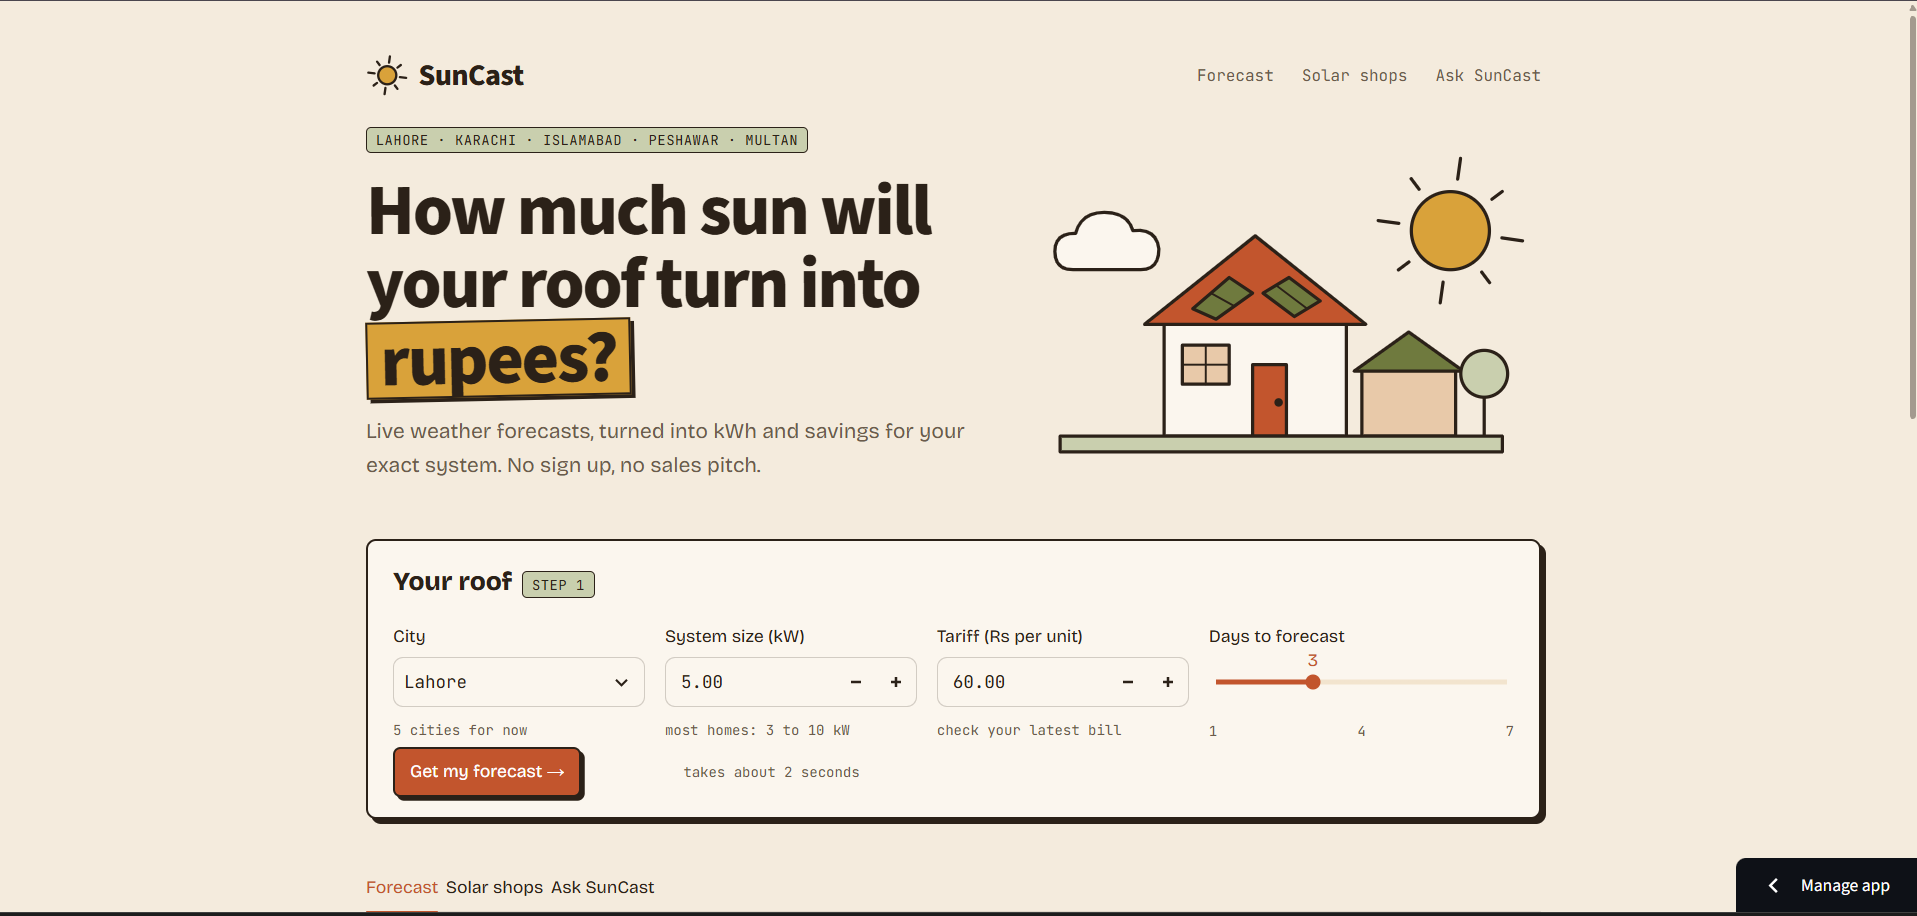
\includegraphics[width=0.9\textwidth]{ui_forcast.png}
\caption{Home page with the inputs card (Lahore, 5 kW, Rs 60 per unit, 3 days).}
\label{fig:ui-forecast}
\end{figure}

\subsection{Forecast View}
After a forecast, the Forecast tab shows the total energy (kWh), the
estimated savings (Rs) and the best day for the chosen period, a tip on the
best hours to run heavy appliances, a daily chart of generation, and an
hourly chart with the physics baseline drawn as a comparison line
(Figure~\ref{fig:ui-forecast2}). A table below gives the numbers for each
day (Figure~\ref{fig:ui-forecast3}).

\begin{figure}[H]
\centering
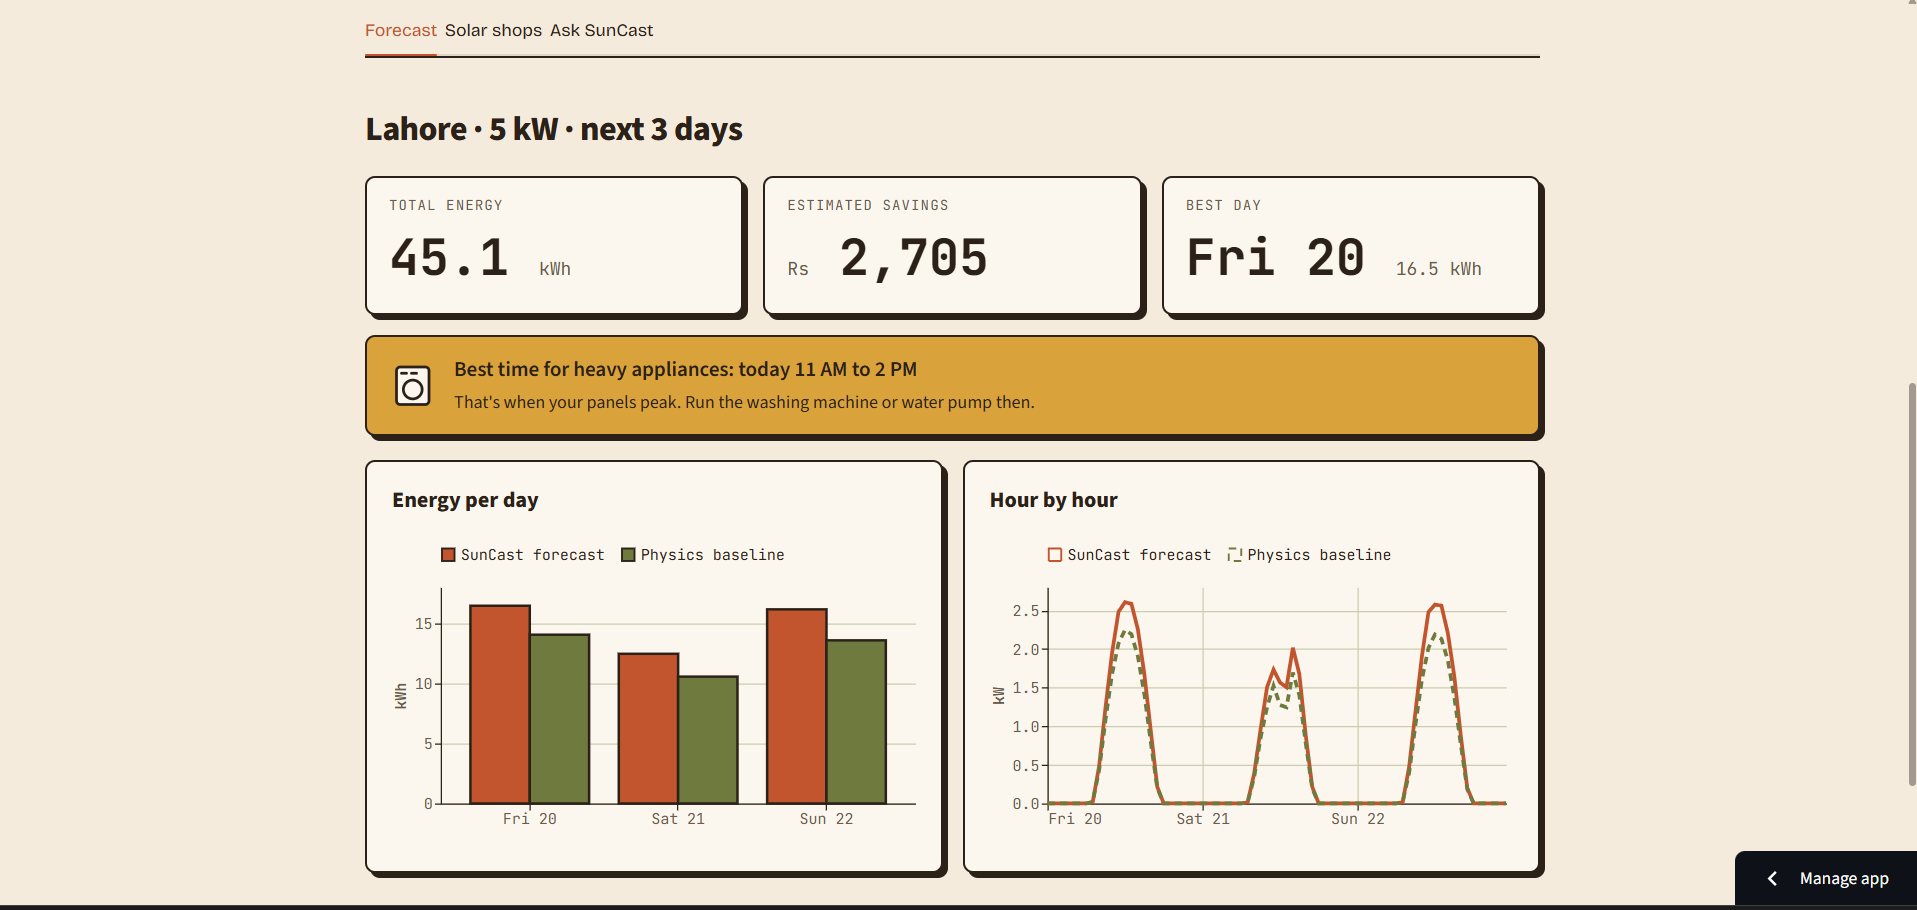
\includegraphics[width=0.9\textwidth]{ui_Forcast2.png}
\caption{Forecast results: total energy, savings, best day, the appliance tip and the daily and hourly charts.}
\label{fig:ui-forecast2}
\end{figure}

\begin{figure}[H]
\centering
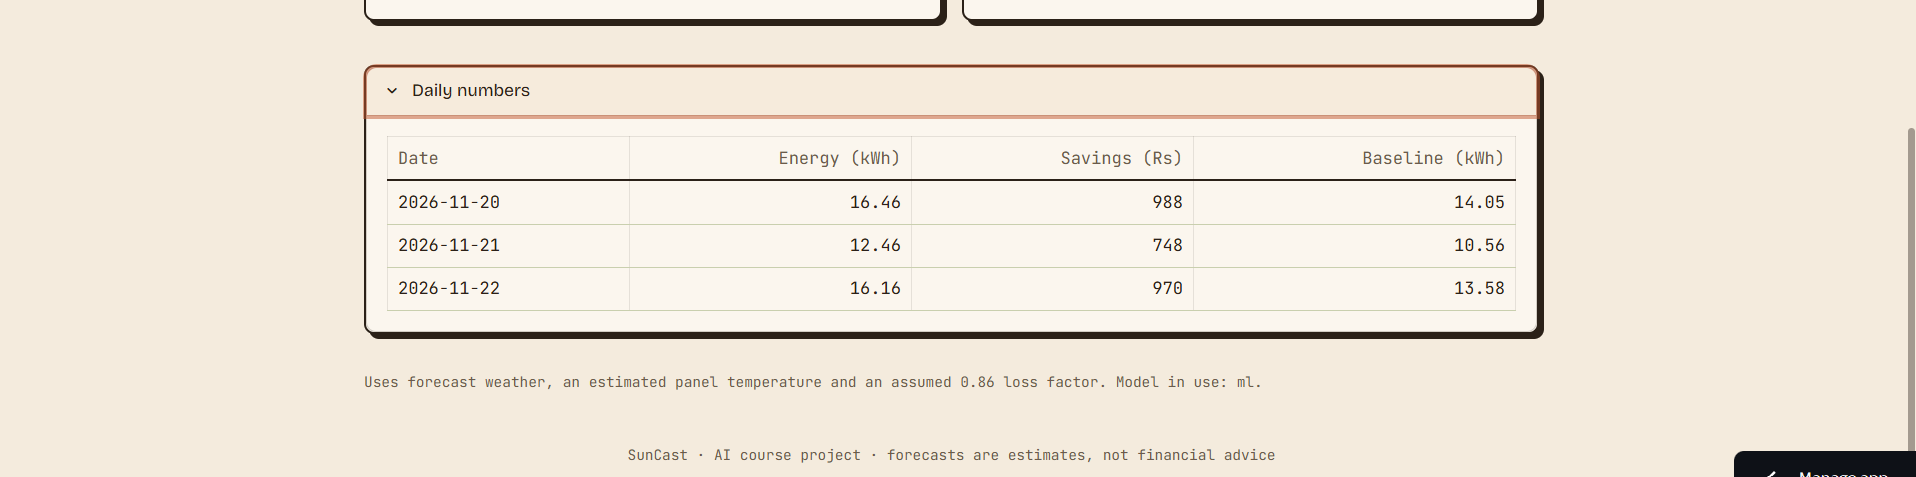
\includegraphics[width=0.9\textwidth]{forcast_ui3.png}
\caption{Daily numbers table.}
\label{fig:ui-forecast3}
\end{figure}

\subsection{Solar Shops}
The Solar shops tab lists retailers in the chosen city with their area,
rating and phone number, taken from the backend
(Figure~\ref{fig:ui-retailers}).

\begin{figure}[H]
\centering
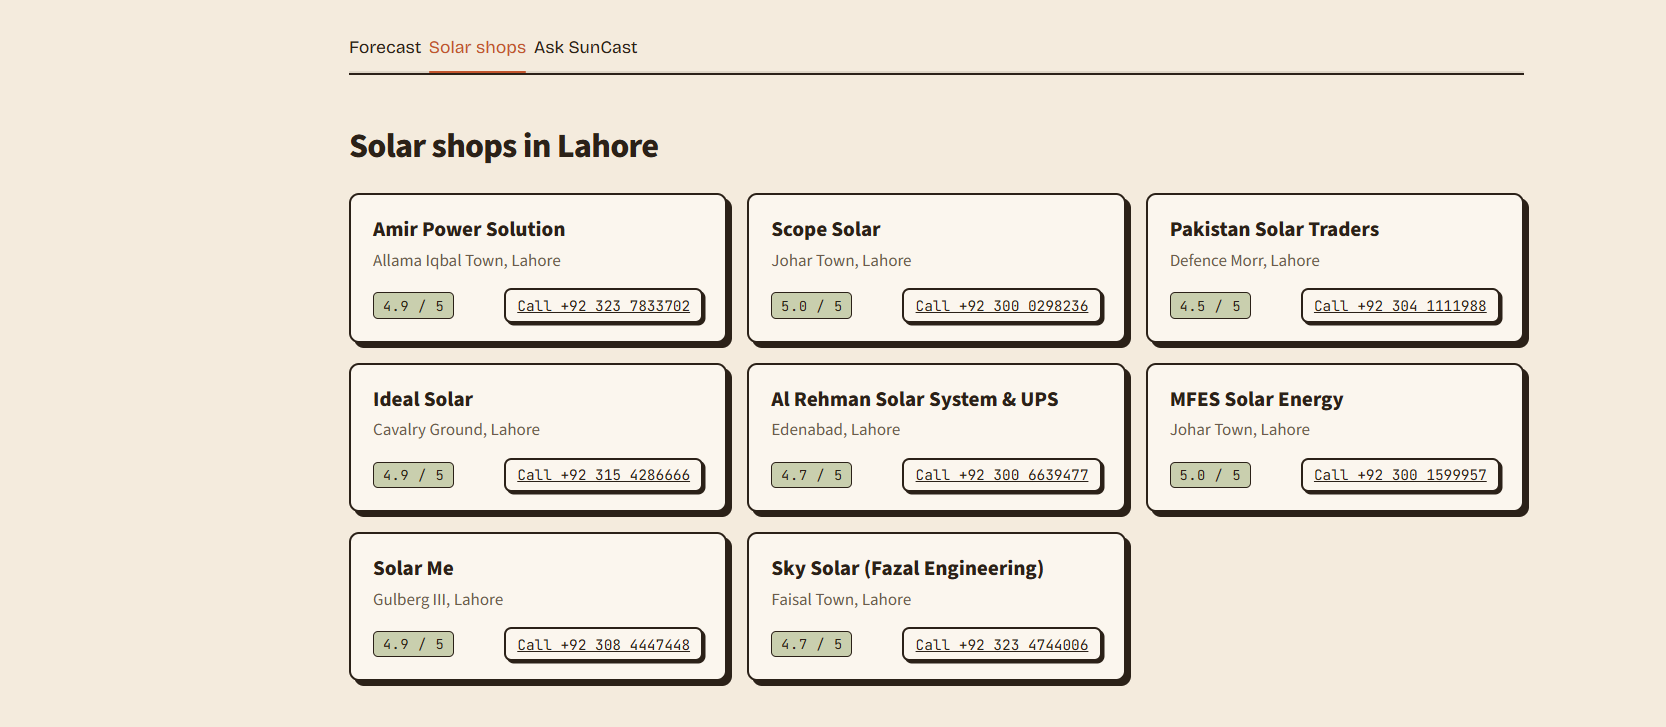
\includegraphics[width=0.9\textwidth]{retailer_ui.png}
\caption{Solar shops in Lahore.}
\label{fig:ui-retailers}
\end{figure}

\subsection{Ask SunCast}
The Ask SunCast tab lets users ask solar questions in plain language, such
as whether a battery is worth it. The question and the selected city are
sent to the backend chatbot, and the reply is shown on the page
(Figure~\ref{fig:ui-chat}).

\begin{figure}[H]
\centering
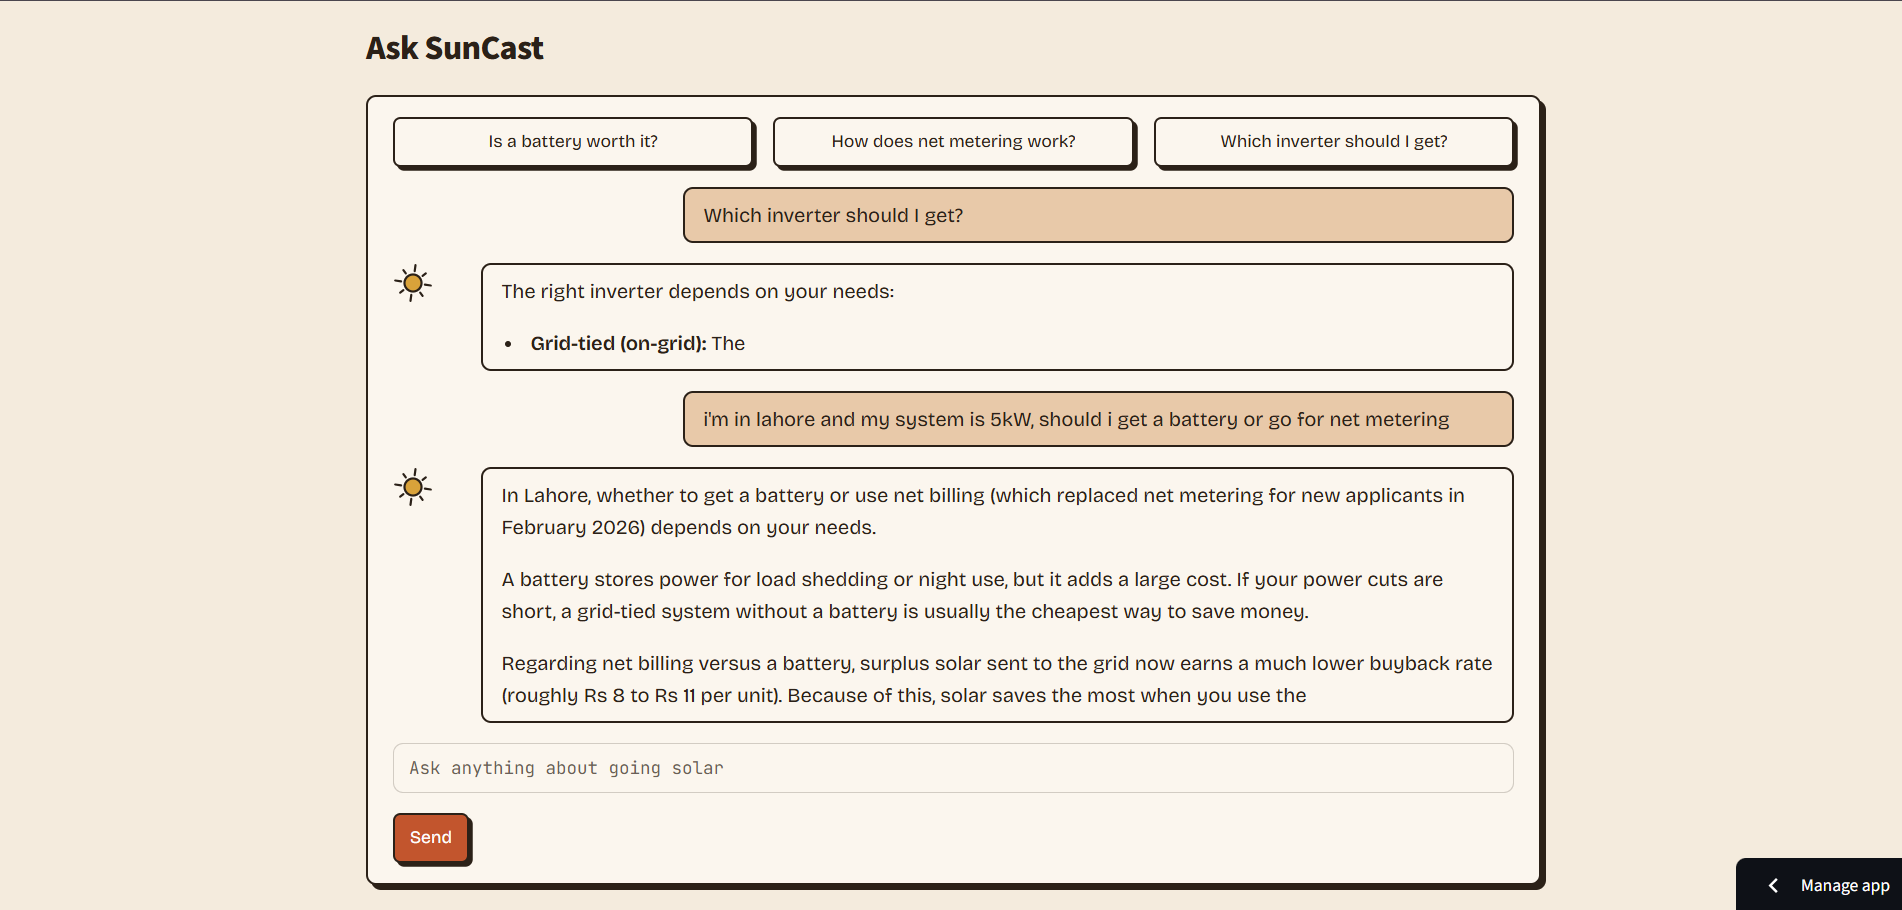
\includegraphics[width=0.9\textwidth]{ui_chat.png}
\caption{Ask SunCast answering a question about batteries and net billing.}
\label{fig:ui-chat}
\end{figure}

\subsection{Design Choices}
We kept everything on one page with three tabs, so a first time buyer is
never shown more than they need. Results use rupees and kWh rather than
technical terms, and the app runs in a mock mode with sample data when no
backend address is set, which let us build the frontend before the backend
was ready.